\documentclass[11pt]{article}
 \usepackage{amsmath}
 \usepackage{hyperref}
 \usepackage{graphicx}
 \usepackage{paralist}
\hypersetup{
    colorlinks,
    citecolor=blue,
    filecolor=blue,
    linkcolor=blue,
    urlcolor=blue
}
\usepackage[top=0.5in, bottom=0.5in, left=0.8in, right=0.8in]{geometry}

 \title{Final Project of CS 177:The Useful Octave package of Finance}
 \author{Huimin Jia \& Kai Wu}
 \begin{document}
  \maketitle
  \begin{abstract}
  This article is mainly based on the introduction of a specified Octave package: Financial. There are several parts included. We will first introduce the installation, and then several most useful functions in this package will be listed. After that,two exercises with solutions have been attached so that it will help readers to understand the package more deeply. 
  \end{abstract}

  \section{Introduction}
    Financial package is a tool used for economic, commercial and stock computing in Octave. It contains many functions such as manipulation and plotting diagrams. Here is the link of the package: \url{http://octave.sourceforge.net/financial/index.html}.You still need to install dependencies package Time(version $>= 1.0.5$) and Miscellaneous(version $>=1.0.6$) before install this. And you need an Octave version after 3.2.4.


  \section{How to install package}
    First go to \url{http://octave.sourceforge.net/packages.php}. By going to the package web page and clicking download. Then start Octave and go to the directory where you placed the downloaded package using the cd command. Then type:
\\\textbf{pkg install package\_file\_name.tar.gz}
\\where package\_file\_name.tar.gz is the file name of the package you downloaded. Than simply type:
\\\textbf{pkg load package\_name} or \textbf{pkg load all}
\\You can get FAQ about install at link: \url{http://octave.sourceforge.net/FAQ.html\#install}.


  \section{Most Useful Functions In the Package}
    \subsection{\_\_fetch\_google\_\_}
$[data,fields]=\_\_fetch\_google\_\_ (conn, symbol, fromdate, todate, period)
\\$This function is used to download stock data from finance.google.com. Output $fields$ is a 1*6 cell that lists names of each data fields about stock in order to explain the 6*6 matrix of output $data$. Include: Date, Open, High, Low, Close, Volume. 
\\
\\var $conn$ should input the function $google()$, using to connect to google, get url "http://finance.google.com". var $symbol$ is the stock name. var $fromdate$ and $ todate$ is the date datenum(serial date number) for the requested date range. If you enter today's date, you will get yesterday's data. var $period$ allows you to select the period for the data which can be "d"(daily) or "w"(weekly).

\subsection{bolling}
$\{\} = bolling (asset, samples)$
\\$\{\} = bolling (asset, samples, alpha)$
\\$\{\} = bolling (asset, samples, alpha, width)$
\\$\{[movavg, upperband, lowerband]\} = bolling (asset, samples, alpha, width)$
\\If no output is requested, function will plot the bollinger bands of the var $asset$. If output is requested, function will return the values for the bollinger bands. 
\\
\\Var $asset$ is Volume came from $\_\_fetch\_google\_\_$. If given, var $alpha$ is the weighting power of the moving average; 0 (default) is the simple moving average.   var $width$ is the number of standard deviations to plot above and below the moving average (default: 2).

\subsection{highlow}
$\{\} = highlow (high, low, close)$
\\$\{\} = highlow (high, low, close, open)$
\\$\{\} = highlow (high, low, close, open, color)$
\\This function is used to plot the var $high$, $low$, and $close$ of a security. The var $close$ is plotted as a tick to the right, and if var $open$ is given and non-empty, it is plotted as a tick to the left.  The color can override the default color for the plot.

\subsection{movavg}
$\{\} = movavg (asset, lead, lag)$
\\$\{\} = movavg (asset, lead, lag, alpha)$
\\$\{[short, long] \} = movavg (asset, lead, lag, alpha)$
\\Calculate the leading and lagging moving average of an asset. If no output is requested the data is plotted.  The plots are drawn in the following order: $asset$, $lag$, $lead$.  If output is requested, no plot is generated, output $short$ and $long$ are x and y of the coordinate system.
\\
\\Var $asset$ is Volume came from $\_\_fetch\_google\_\_$, $lead$ is the leading stock,  $lag$ is the lagging stock. If given, var $alpha$ is the weighting power of the delay; 0 (default) is the simple moving average, 0.5 would be the square root weighted moving average, 1 would be linear, 2 would be squared, ..., and 'e' is the exponential moving average.

\subsection{pointfig}
$\{\} = pointfig (asset)$
\\ This function is used for plotting the point figure chart of an asset. In the chart, the upward price movements are plotted as Xs, while downward movements are plotted as Os.

\subsection{posvolidx and negvolidx}
$\{pvi\} = posvolidx (c, vol, initpvi)$
$\{nvi\} = negvolidx (c, vol, initpvi)$
\\ This function is used for computing the positive(negative) volume index of a security based on its closing price and volume.

\subsection{onbalvol}
$\{obv\} = posvolidx (c, vol)$
\\ This function is used for computing the on balance volume of a security based on its closing price and volume. The output will be a column vector, and the first number in the output is always 0.

\subsection{pmt}
$\{\} = pmt (r, n, a, l, m)$
\\ Return the amount of periodic payment necessary to amortize a loan of amount a with interest rate var $r$ in $n$ periods.
\\
\\The optional argument var $l$ may be used to specify a terminal lump-sum payment. The optional argument var $m$ may be used to specify whether payments are made at the end, "e"(default) or "b"(at the beginning) of each period.

\subsection{mirr}
$rate = mirr (flow, finrate, reinvestrate)$
\\ Compute the modified internal rate of return. Take periodic cashflows as a vector and the finance rate,
\\Var $finrate$, for negative cash flows and a reinvestment rate, $reinvestrate$, for positive cash flows.

\section{Exercise}
\subsection{Problem 1}
Link to finance.google.com and retrieve the datasets of yahoo from Jan.1st,2010 to Mar.15th, 2010. Then give the plotting work as shown below:

\begin{enumerate}[{[}1{]}]
\item Plot the bolling curve of the volume during this time period, using the simple moving average with both upper band and lower band.
\item Plot the highlow curve for this datasets.
\item Plot the moving average curve for the closed prices during this time period, giving 3 leading samples and 20 lagging samples.
\item Plot both upward \& downward trend of the closed prices.
\end{enumerate}

\subsection{Problem 2}
Using the dataset from Exercise 1, do the following computing work:
\begin{enumerate}[{[}1{]}]
\item Compute both the positive volume index and negative volume index of a security based on the closing price and volume, assuming that the starting value of the pvi and nvi is 100. Also, give the on balance volume of a security based on the closing price and volume.
\item Assuming that one company has borrowed 100,000 from the bank at the rate of 2.5% per month, compute how much it have to pay back monthly to the bank in 1 year. Compare the two conditions which are paid at the beginning of the month and at the end of the month.
\item A set of data about the cash flow was given from the year 2000 to 2010,which are 30,000 -10,000 50,000, 100,000,-40,000 -80,000 35,000 -50.000 -65,000 15,000. Compute the modified internal rate of return, assuming that the finrate value= 0.05 and the reinvestrate value = 0.03.
\end{enumerate}


\section{Solutions}
\subsection{Solutions for problem 1}
$a = datenum(2010,1,1);b = datenum(2010,3,15);$
\\$[d,f]= \_\_fetch\_google\_\_(google(), ”yhoo”, a, b, "d");$
\begin{enumerate}[{[}1{]}] 
\item $Bolling(d(:,6),2,0,2)$ (See Chart 1)
\item $highlow(d(:,3),d(:,4),d(:,5),d(:,2))$ (See Chart 2)
\item $movavg(d(:,5),3,20,0)$ (See Chart 3)
\item $pointfig(d(:,5))$ (See Chart 4)
\end{enumerate}

 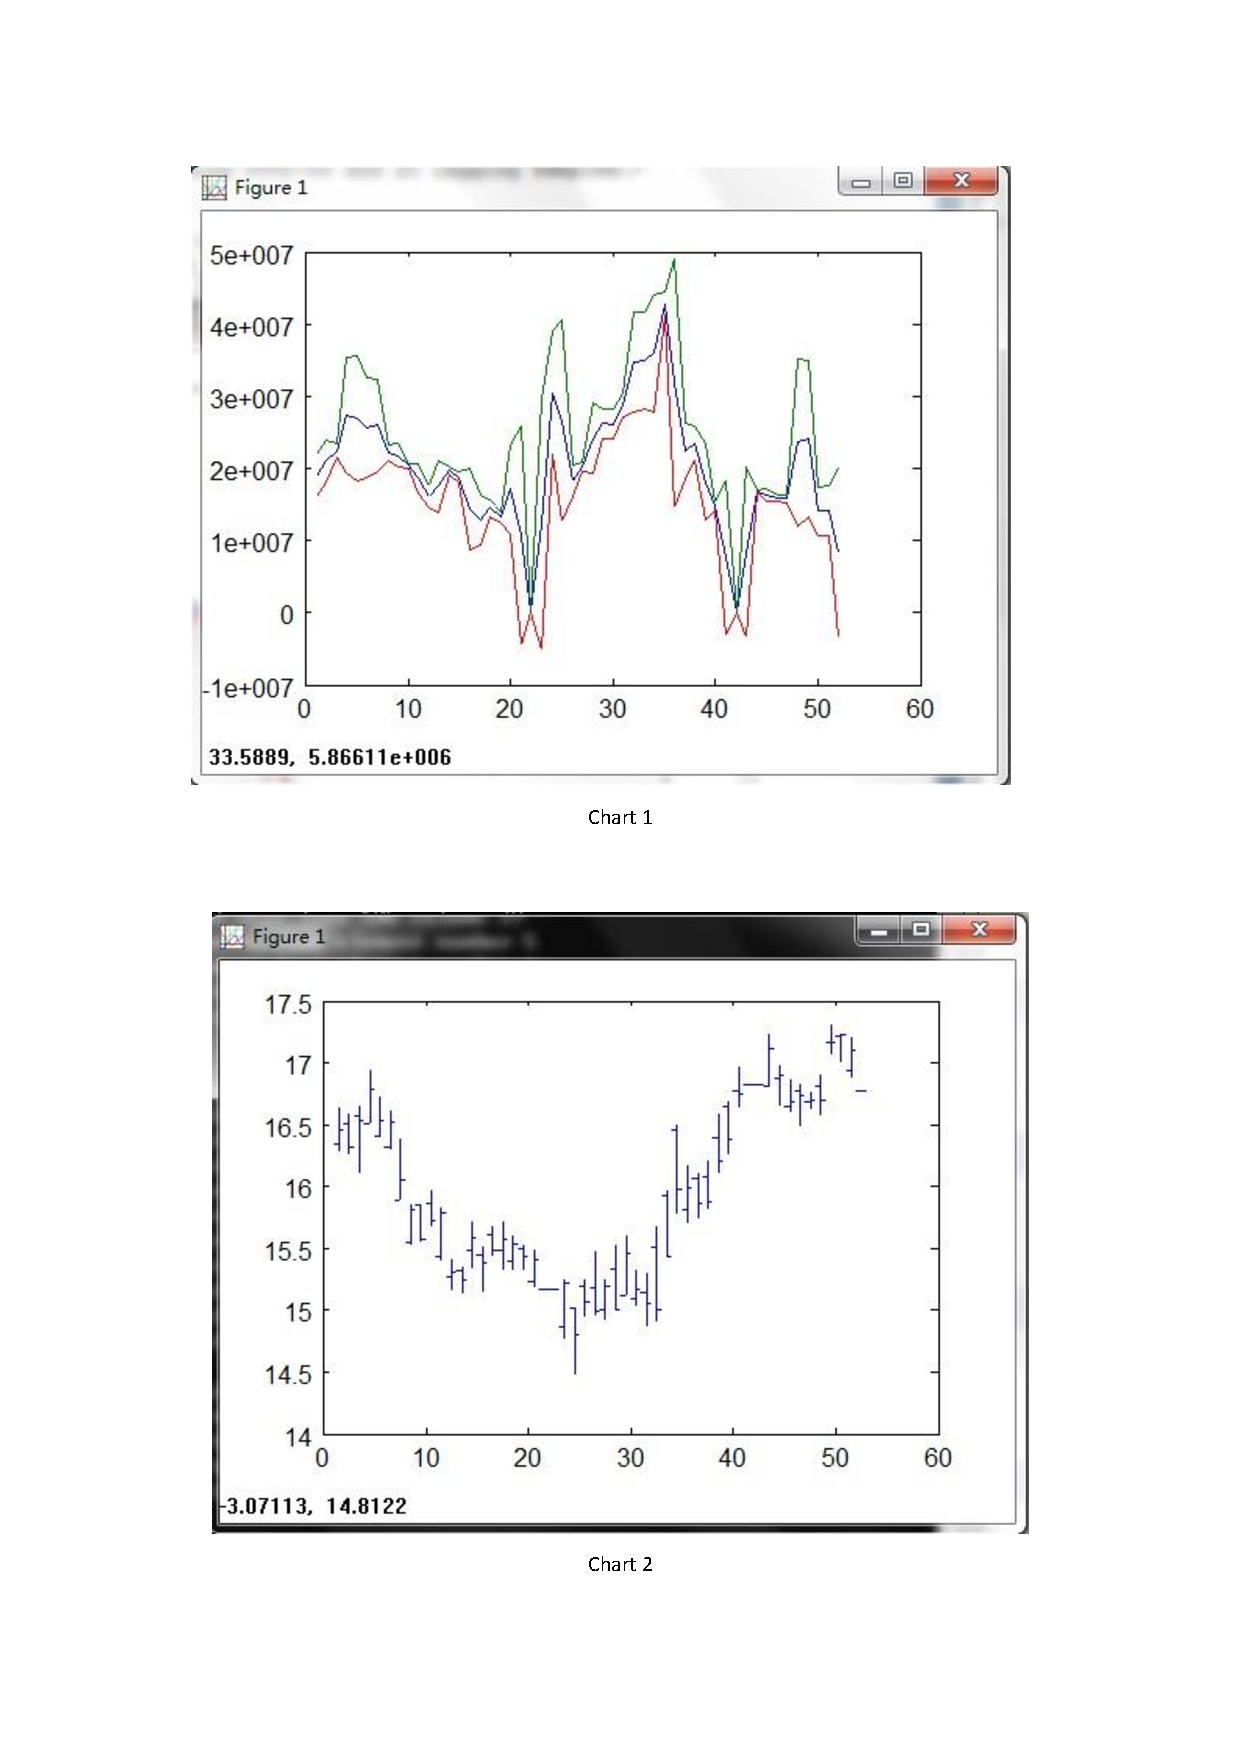
\includegraphics[scale=0.4]{Doc1}
 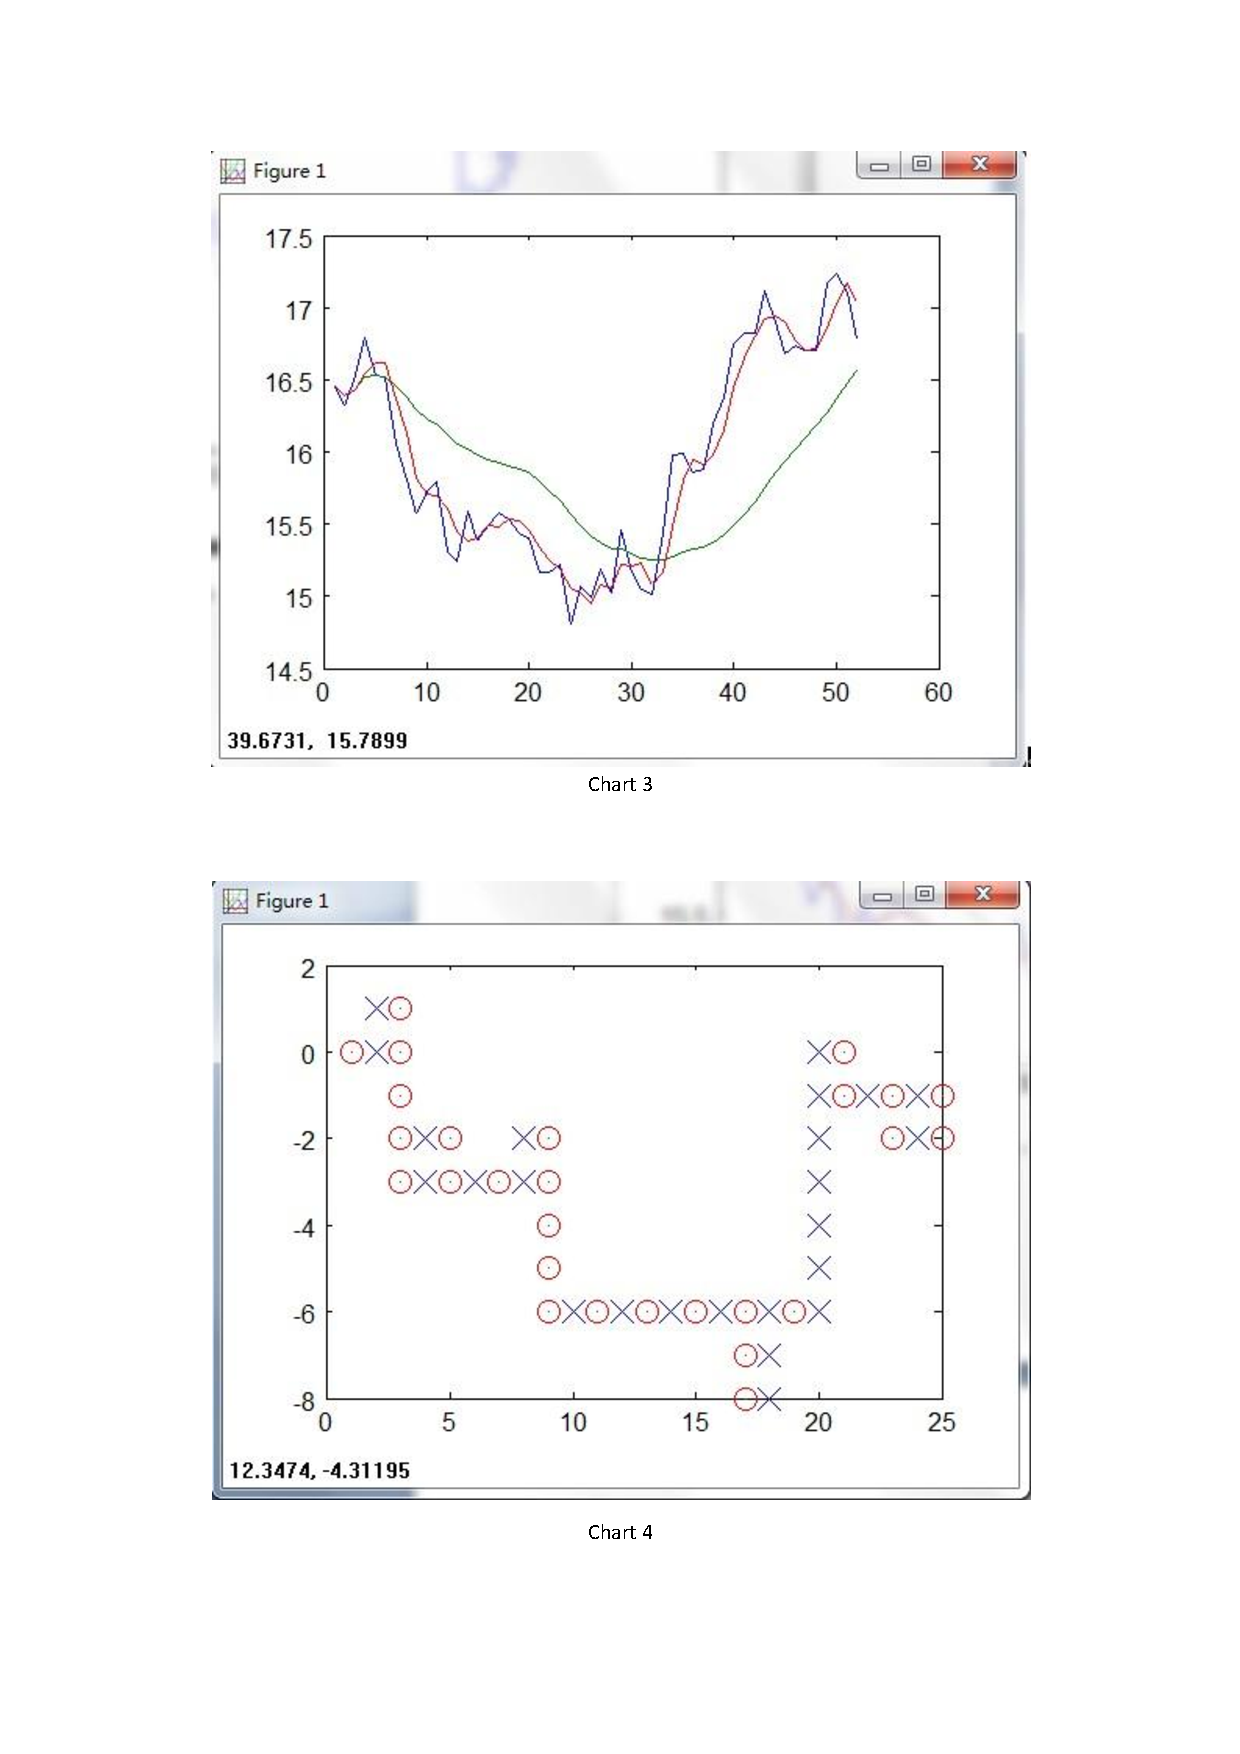
\includegraphics[scale=0.4]{Doc2}

\subsection{Solutions for problem 2}
\begin{enumerate}[{[}1{]}] 
\item posvolidx(d(:,5),d(:,6),100); negvolidx(d(:,5),d(:,6),100); onbalvol(d(:,5),d(:,6),100)
\item pmt(0.025,12,100000,”b”); pmt(0.025,12,100000,”e”)
\item mirr([30000 -10000 50000 100000 -40000 -80000 35000 -50000 -65000 15000],0.05,0.03)
\end{enumerate}

\section{Conclusion}
After the problem-solving process with several functions in financial package, I think readers are able to be more familiar with the use of package. The process of applying them to the financial model curve plotting and computing would be very helpful. However, there are still many other functions not mentioned in this project. We strongly encourage you to check those files and see whether it is useful for your later study life. 

\begin{thebibliography}{9}

\bibitem{Knuth92} The octave financial package, available at:
\\{\tt \url{http://octave.sourceforge.net/financial/index.htmll}.}

\bibitem{Knuth92} The stock data from Google Finance, available at:
\\{\tt \url{http://finance.google.com}.}

\end{thebibliography}
 \end{document}